\documentclass{article}\usepackage[]{graphicx}\usepackage[]{color}
%% maxwidth is the original width if it is less than linewidth
%% otherwise use linewidth (to make sure the graphics do not exceed the margin)
\makeatletter
\def\maxwidth{ %
  \ifdim\Gin@nat@width>\linewidth
    \linewidth
  \else
    \Gin@nat@width
  \fi
}
\makeatother

\definecolor{fgcolor}{rgb}{0.345, 0.345, 0.345}
\newcommand{\hlnum}[1]{\textcolor[rgb]{0.686,0.059,0.569}{#1}}%
\newcommand{\hlstr}[1]{\textcolor[rgb]{0.192,0.494,0.8}{#1}}%
\newcommand{\hlcom}[1]{\textcolor[rgb]{0.678,0.584,0.686}{\textit{#1}}}%
\newcommand{\hlopt}[1]{\textcolor[rgb]{0,0,0}{#1}}%
\newcommand{\hlstd}[1]{\textcolor[rgb]{0.345,0.345,0.345}{#1}}%
\newcommand{\hlkwa}[1]{\textcolor[rgb]{0.161,0.373,0.58}{\textbf{#1}}}%
\newcommand{\hlkwb}[1]{\textcolor[rgb]{0.69,0.353,0.396}{#1}}%
\newcommand{\hlkwc}[1]{\textcolor[rgb]{0.333,0.667,0.333}{#1}}%
\newcommand{\hlkwd}[1]{\textcolor[rgb]{0.737,0.353,0.396}{\textbf{#1}}}%

\usepackage{framed}
\makeatletter
\newenvironment{kframe}{%
 \def\at@end@of@kframe{}%
 \ifinner\ifhmode%
  \def\at@end@of@kframe{\end{minipage}}%
  \begin{minipage}{\columnwidth}%
 \fi\fi%
 \def\FrameCommand##1{\hskip\@totalleftmargin \hskip-\fboxsep
 \colorbox{shadecolor}{##1}\hskip-\fboxsep
     % There is no \\@totalrightmargin, so:
     \hskip-\linewidth \hskip-\@totalleftmargin \hskip\columnwidth}%
 \MakeFramed {\advance\hsize-\width
   \@totalleftmargin\z@ \linewidth\hsize
   \@setminipage}}%
 {\par\unskip\endMakeFramed%
 \at@end@of@kframe}
\makeatother

\definecolor{shadecolor}{rgb}{.97, .97, .97}
\definecolor{messagecolor}{rgb}{0, 0, 0}
\definecolor{warningcolor}{rgb}{1, 0, 1}
\definecolor{errorcolor}{rgb}{1, 0, 0}
\newenvironment{knitrout}{}{} % an empty environment to be redefined in TeX

\usepackage{alltt}

\usepackage{booktabs}
\IfFileExists{upquote.sty}{\usepackage{upquote}}{}
\begin{document}






\begin{knitrout}
\definecolor{shadecolor}{rgb}{0.969, 0.969, 0.969}\color{fgcolor}\begin{kframe}
\begin{alltt}
\hlkwd{setPar}\hlstd{()}
\hlkwd{plot}\hlstd{(SelAByYear,} \hlkwc{x}\hlstd{=}\hlnum{2006}\hlopt{:}\hlnum{2015}\hlstd{,} \hlkwc{ylim}\hlstd{=}\hlkwd{c}\hlstd{(}\hlkwd{min}\hlstd{( CISelAByYear),} \hlkwd{max}\hlstd{( CISelAByYear)),} \hlkwc{xlab}\hlstd{=}\hlstr{"Year"}\hlstd{,} \hlkwc{ylab} \hlstd{=} \hlstr{"Selection gradient"}\hlstd{,} \hlkwc{main} \hlstd{=} \hlstr{"\textbackslash{}\textbackslash{}textbf\{(A)\} Total selection"}\hlstd{)}
\hlkwd{abline}\hlstd{(}\hlkwc{h}\hlstd{=}\hlnum{0}\hlstd{)}
\hlkwd{arrows}\hlstd{(}\hlkwc{x0} \hlstd{=} \hlnum{2006}\hlopt{:}\hlnum{2015}\hlstd{,}\hlkwc{x1} \hlstd{=} \hlnum{2006}\hlopt{:}\hlnum{2015}\hlstd{,}\hlkwc{code} \hlstd{=} \hlnum{3}\hlstd{,} \hlkwc{y0} \hlstd{= CISelAByYear[}\hlnum{1}\hlstd{,],}
       \hlkwc{y1} \hlstd{= CISelAByYear[}\hlnum{2}\hlstd{,],} \hlkwc{angle} \hlstd{=} \hlnum{90}\hlstd{,}\hlkwc{length} \hlstd{=} \hlnum{0.1}\hlstd{)}
\hlkwd{abline}\hlstd{(}\hlkwc{h}\hlstd{=}\hlkwd{coefficients}\hlstd{(m0all)[}\hlnum{2}\hlstd{],} \hlkwc{lty}\hlstd{=}\hlnum{2}\hlstd{,} \hlkwc{lwd}\hlstd{=}\hlnum{5}\hlstd{)}
\hlstd{lowm0all} \hlkwb{<-} \hlkwd{coefficients}\hlstd{(m0all)[}\hlnum{2}\hlstd{]}\hlopt{+}\hlnum{1.96}\hlopt{*}\hlstd{sm0all}\hlopt{$}\hlstd{coefficients[}\hlnum{2}\hlstd{,}\hlnum{2}\hlstd{]}
\hlstd{highm0all} \hlkwb{<-} \hlkwd{coefficients}\hlstd{(m0all)[}\hlnum{2}\hlstd{]}\hlopt{-}\hlnum{1.96}\hlopt{*}\hlstd{sm0all}\hlopt{$}\hlstd{coefficients[}\hlnum{2}\hlstd{,}\hlnum{2}\hlstd{]}
\hlkwd{polygon}\hlstd{(}\hlkwc{x}\hlstd{=}\hlkwd{c}\hlstd{(}\hlnum{2005}\hlstd{,}\hlnum{2016}\hlstd{,}\hlnum{2016}\hlstd{,}\hlnum{2005}\hlstd{),}\hlkwc{y}\hlstd{=}\hlkwd{c}\hlstd{(lowm0all,lowm0all, highm0all, highm0all),}
        \hlkwc{fillOddEven} \hlstd{=} \hlnum{TRUE}\hlstd{,} \hlkwc{col}\hlstd{=}\hlkwd{rgb}\hlstd{(}\hlnum{0.1}\hlstd{,}\hlnum{0.1}\hlstd{,}\hlnum{0.1}\hlstd{,}\hlnum{0.3}\hlstd{),} \hlkwc{lty}\hlstd{=}\hlnum{2}\hlstd{)}
\end{alltt}
\end{kframe}
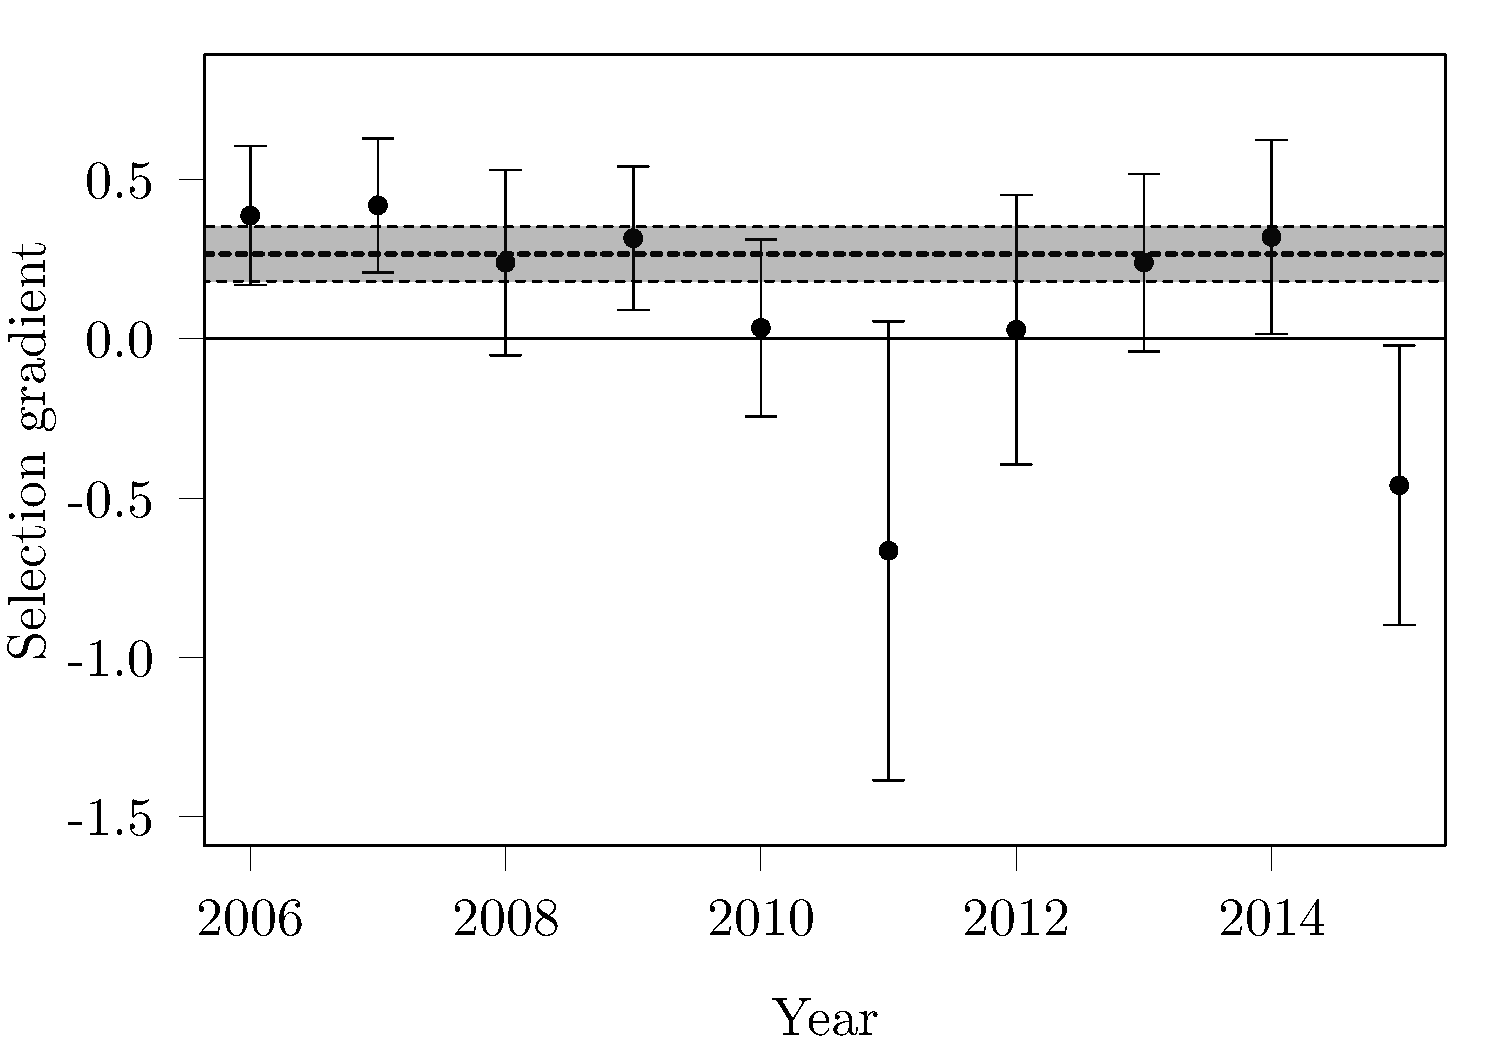
\includegraphics[width=\maxwidth]{figure/SelByYear-1} 
\begin{kframe}\begin{alltt}
\hlcom{#points(x=2006:2015,y=unlist(coefficients(mmRnoCorfitness)$Year["StMass"]), pch=17)}
\end{alltt}
\end{kframe}
\end{knitrout}

\begin{knitrout}
\definecolor{shadecolor}{rgb}{0.969, 0.969, 0.969}\color{fgcolor}\begin{kframe}
\begin{alltt}
\hlkwd{setPar}\hlstd{()}
\hlkwd{plot}\hlstd{(SelAByYearRho,} \hlkwc{x}\hlstd{=}\hlnum{2006}\hlopt{:}\hlnum{2015}\hlstd{,} \hlkwc{ylim}\hlstd{=}\hlkwd{c}\hlstd{(}\hlkwd{min}\hlstd{( CISelAByYearRho),} \hlkwd{max}\hlstd{( CISelAByYearRho)),} \hlkwc{xlab}\hlstd{=}\hlstr{"Year"}\hlstd{,} \hlkwc{ylab} \hlstd{=} \hlstr{"Selection gradient on $\textbackslash{}\textbackslash{}rho$"}\hlstd{,} \hlkwc{main} \hlstd{=} \hlstr{"\textbackslash{}\textbackslash{}textbf\{(B)\} Fertility selection"}\hlstd{)}
\hlkwd{abline}\hlstd{(}\hlkwc{h}\hlstd{=}\hlnum{0}\hlstd{)}
\hlkwd{arrows}\hlstd{(}\hlkwc{x0} \hlstd{=} \hlnum{2006}\hlopt{:}\hlnum{2015}\hlstd{,}\hlkwc{x1} \hlstd{=} \hlnum{2006}\hlopt{:}\hlnum{2015}\hlstd{,}\hlkwc{code} \hlstd{=} \hlnum{3}\hlstd{,} \hlkwc{y0} \hlstd{= CISelAByYearRho[}\hlnum{1}\hlstd{,],}
       \hlkwc{y1} \hlstd{= CISelAByYearRho[}\hlnum{2}\hlstd{,],} \hlkwc{angle} \hlstd{=} \hlnum{90}\hlstd{,}\hlkwc{length} \hlstd{=} \hlnum{0.1}\hlstd{)}
\hlkwd{abline}\hlstd{(}\hlkwc{h}\hlstd{=}\hlkwd{coefficients}\hlstd{(m0allRho)[}\hlnum{2}\hlstd{],} \hlkwc{lty}\hlstd{=}\hlnum{2}\hlstd{)}
\hlstd{sm0allRho} \hlkwb{<-} \hlkwd{summary}\hlstd{(m0allRho)}
\hlstd{lowm0allRho} \hlkwb{<-} \hlkwd{coefficients}\hlstd{(m0allRho)[}\hlnum{2}\hlstd{]}\hlopt{+}\hlnum{1.96}\hlopt{*}\hlstd{sm0allRho}\hlopt{$}\hlstd{coefficients[}\hlnum{2}\hlstd{,}\hlnum{2}\hlstd{]}
\hlstd{highm0allRho} \hlkwb{<-} \hlkwd{coefficients}\hlstd{(m0allRho)[}\hlnum{2}\hlstd{]}\hlopt{-}\hlnum{1.96}\hlopt{*}\hlstd{sm0allRho}\hlopt{$}\hlstd{coefficients[}\hlnum{2}\hlstd{,}\hlnum{2}\hlstd{]}
\hlkwd{polygon}\hlstd{(}\hlkwc{x}\hlstd{=}\hlkwd{c}\hlstd{(}\hlnum{2005}\hlstd{,}\hlnum{2016}\hlstd{,}\hlnum{2016}\hlstd{,}\hlnum{2005}\hlstd{),}\hlkwc{y}\hlstd{=}\hlkwd{c}\hlstd{(lowm0allRho,lowm0allRho, highm0allRho, highm0allRho),}
        \hlkwc{fillOddEven} \hlstd{=} \hlnum{TRUE}\hlstd{,} \hlkwc{col}\hlstd{=}\hlkwd{rgb}\hlstd{(}\hlnum{0.1}\hlstd{,}\hlnum{0.1}\hlstd{,}\hlnum{0.1}\hlstd{,}\hlnum{0.5}\hlstd{),} \hlkwc{lty}\hlstd{=}\hlnum{2}\hlstd{)}
\end{alltt}
\end{kframe}
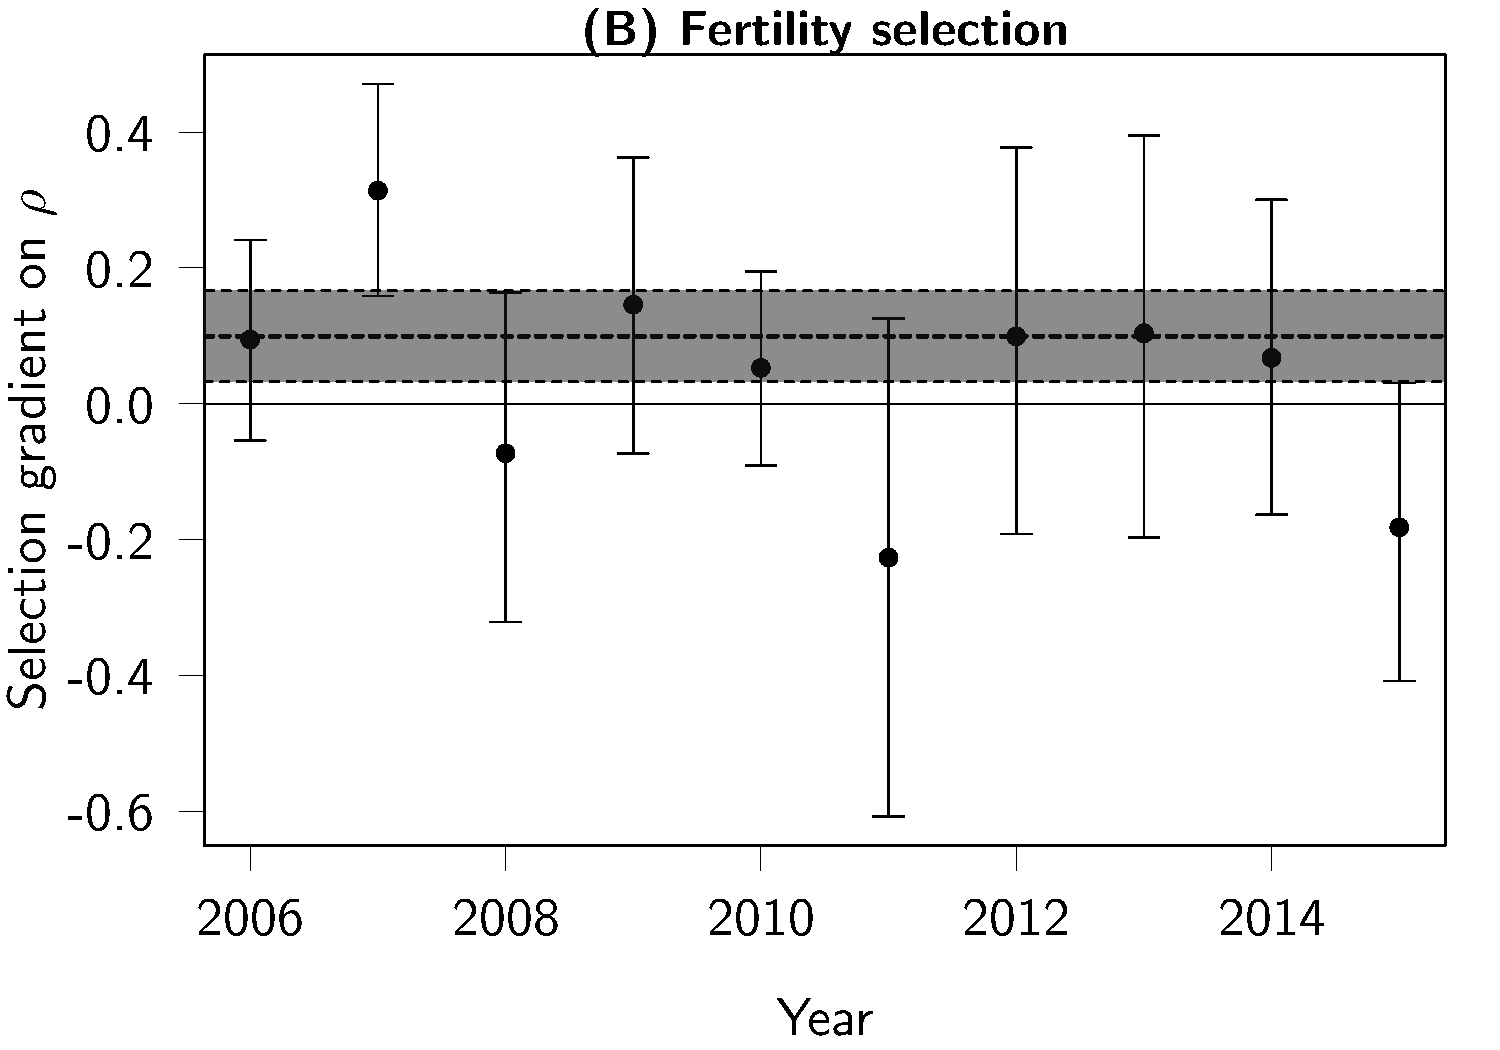
\includegraphics[width=\maxwidth]{figure/SelByYearRho-1} 

\end{knitrout}


\begin{knitrout}
\definecolor{shadecolor}{rgb}{0.969, 0.969, 0.969}\color{fgcolor}\begin{kframe}
\begin{alltt}
\hlkwd{setPar}\hlstd{()}
\hlkwd{plot}\hlstd{(SelAByYearPhi,} \hlkwc{x}\hlstd{=}\hlnum{2006}\hlopt{:}\hlnum{2015}\hlstd{,} \hlkwc{ylim}\hlstd{=}\hlkwd{c}\hlstd{(}\hlkwd{min}\hlstd{( CISelAByYearPhi,} \hlkwc{na.rm}\hlstd{=}\hlnum{TRUE}\hlstd{),} \hlkwd{max}\hlstd{( CISelAByYearPhi,} \hlkwc{na.rm}\hlstd{=}\hlnum{TRUE}\hlstd{)),} \hlkwc{xlab}\hlstd{=}\hlstr{"Year"}\hlstd{,} \hlkwc{ylab} \hlstd{=} \hlstr{"Selection gradient on $\textbackslash{}\textbackslash{}phi$"}\hlstd{,} \hlkwc{main} \hlstd{=} \hlstr{"\textbackslash{}\textbackslash{}textbf\{(C)\} Viability selection"}\hlstd{)}
\hlkwd{abline}\hlstd{(}\hlkwc{h}\hlstd{=}\hlnum{0}\hlstd{)}
\hlkwd{arrows}\hlstd{(}\hlkwc{x0} \hlstd{=} \hlnum{2006}\hlopt{:}\hlnum{2015}\hlstd{,}\hlkwc{x1} \hlstd{=} \hlnum{2006}\hlopt{:}\hlnum{2015}\hlstd{,}\hlkwc{code} \hlstd{=} \hlnum{3}\hlstd{,} \hlkwc{y0} \hlstd{= CISelAByYearPhi[}\hlnum{1}\hlstd{,],}
       \hlkwc{y1} \hlstd{= CISelAByYearPhi[}\hlnum{2}\hlstd{,],} \hlkwc{angle} \hlstd{=} \hlnum{90}\hlstd{,}\hlkwc{length} \hlstd{=} \hlnum{0.1}\hlstd{)}
\hlkwd{abline}\hlstd{(}\hlkwc{h}\hlstd{=}\hlkwd{coefficients}\hlstd{(m0allphi)[}\hlnum{2}\hlstd{],} \hlkwc{lty}\hlstd{=}\hlnum{2}\hlstd{)}
\hlstd{lowm0allphi} \hlkwb{<-} \hlkwd{coefficients}\hlstd{(m0allphi)[}\hlnum{2}\hlstd{]}\hlopt{+}\hlnum{1.96}\hlopt{*}\hlstd{sm0allphi}\hlopt{$}\hlstd{coefficients[}\hlnum{2}\hlstd{,}\hlnum{2}\hlstd{]}
\hlstd{highm0allphi} \hlkwb{<-} \hlkwd{coefficients}\hlstd{(m0allphi)[}\hlnum{2}\hlstd{]}\hlopt{-}\hlnum{1.96}\hlopt{*}\hlstd{sm0allphi}\hlopt{$}\hlstd{coefficients[}\hlnum{2}\hlstd{,}\hlnum{2}\hlstd{]}
\hlkwd{polygon}\hlstd{(}\hlkwc{x}\hlstd{=}\hlkwd{c}\hlstd{(}\hlnum{2005}\hlstd{,}\hlnum{2016}\hlstd{,}\hlnum{2016}\hlstd{,}\hlnum{2005}\hlstd{),}\hlkwc{y}\hlstd{=}\hlkwd{c}\hlstd{(lowm0allphi,lowm0allphi, highm0allphi, highm0allphi),}
        \hlkwc{fillOddEven} \hlstd{=} \hlnum{TRUE}\hlstd{,} \hlkwc{col}\hlstd{=}\hlkwd{rgb}\hlstd{(}\hlnum{0.1}\hlstd{,}\hlnum{0.1}\hlstd{,}\hlnum{0.1}\hlstd{,}\hlnum{0.5}\hlstd{),} \hlkwc{lty}\hlstd{=}\hlnum{2} \hlstd{)}
\end{alltt}
\end{kframe}
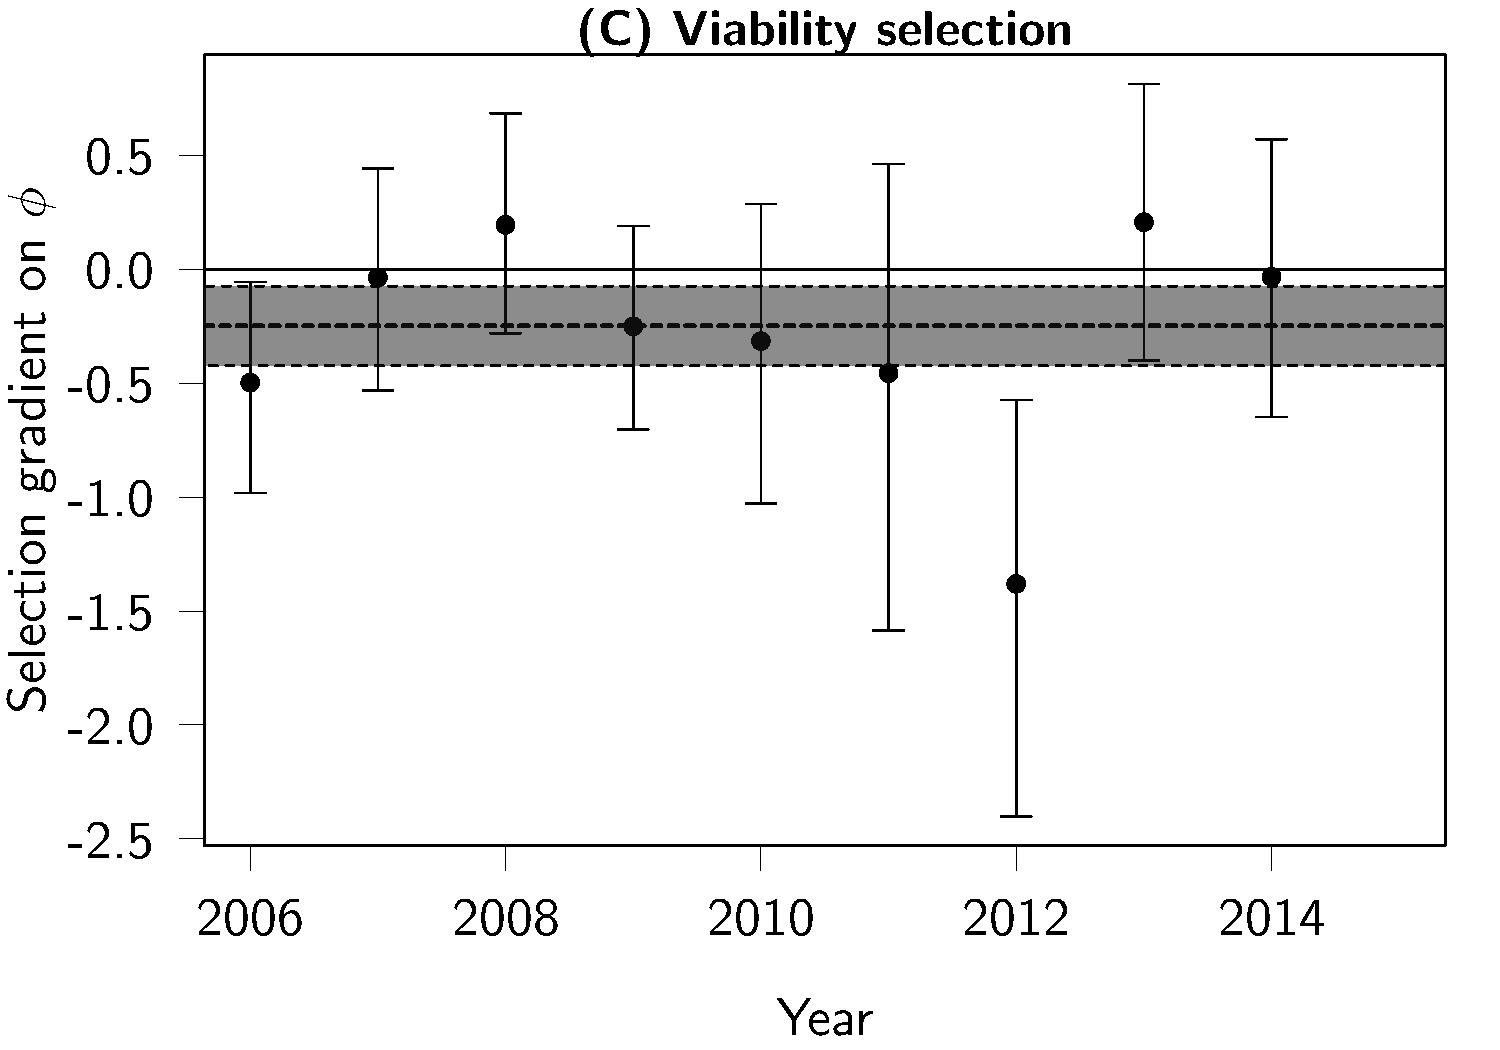
\includegraphics[width=\maxwidth]{figure/SelByYearPhi-1} 

\end{knitrout}
Correlation fertility viability
\begin{knitrout}
\definecolor{shadecolor}{rgb}{0.969, 0.969, 0.969}\color{fgcolor}\begin{kframe}
\begin{alltt}
\hlkwd{cor.test}\hlstd{(YearPheno}\hlopt{$}\hlstd{Phi,YearPheno}\hlopt{$}\hlstd{Rho)}
\end{alltt}
\begin{verbatim}
## 
## 	Pearson's product-moment correlation
## 
## data:  YearPheno$Phi and YearPheno$Rho
## t = -1.9473, df = 1292, p-value = 0.05171
## alternative hypothesis: true correlation is not equal to 0
## 95 percent confidence interval:
##  -0.1082724891  0.0003989614
## sample estimates:
##         cor 
## -0.05409695
\end{verbatim}
\end{kframe}
\end{knitrout}

\begin{knitrout}
\definecolor{shadecolor}{rgb}{0.969, 0.969, 0.969}\color{fgcolor}\begin{kframe}
\begin{alltt}
\hlkwd{sd}\hlstd{(SelByYear)}
\end{alltt}


{\ttfamily\noindent\bfseries\color{errorcolor}{\#\# Error in is.data.frame(x): objet 'SelByYear' introuvable}}\begin{alltt}
\hlkwd{coefficients}\hlstd{(m0all)[}\hlnum{2}\hlstd{]}
\end{alltt}
\begin{verbatim}
##        Ast 
## 0.08200326
\end{verbatim}
\begin{alltt}
\hlkwd{summary}\hlstd{(m0all)[}\hlnum{2}\hlstd{]}
\end{alltt}
\begin{verbatim}
## $terms
## Fitness ~ 1 + Ast + Sex + Age
## attr(,"variables")
## list(Fitness, Ast, Sex, Age)
## attr(,"factors")
##         Ast Sex Age
## Fitness   0   0   0
## Ast       1   0   0
## Sex       0   1   0
## Age       0   0   1
## attr(,"term.labels")
## [1] "Ast" "Sex" "Age"
## attr(,"order")
## [1] 1 1 1
## attr(,"intercept")
## [1] 1
## attr(,"response")
## [1] 1
## attr(,".Environment")
## <environment: R_GlobalEnv>
## attr(,"predvars")
## list(Fitness, Ast, Sex, Age)
## attr(,"dataClasses")
##   Fitness       Ast       Sex       Age 
## "numeric" "numeric"  "factor"  "factor"
\end{verbatim}
\begin{alltt}
\hlkwd{mean}\hlstd{(SeSelByYear)}
\end{alltt}


{\ttfamily\noindent\bfseries\color{errorcolor}{\#\# Error in mean(SeSelByYear): objet 'SeSelByYear' introuvable}}\begin{alltt}
\hlstd{sm0all}
\end{alltt}
\begin{verbatim}
## 
## Call:
## glm(formula = Fitness ~ 1 + Ast + Sex + Age, family = quasipoisson, 
##     data = YearPheno)
## 
## Deviance Residuals: 
##     Min       1Q   Median       3Q      Max  
## -2.8453  -1.0854  -1.0421   0.8231   4.7406  
## 
## Coefficients:
##             Estimate Std. Error t value Pr(>|t|)    
## (Intercept)  1.05005    0.04408  23.822  < 2e-16 ***
## Ast          0.08200    0.02837   2.890  0.00391 ** 
## SexMale     -0.06908    0.06832  -1.011  0.31213    
## AgeJ        -1.56364    0.08072 -19.372  < 2e-16 ***
## ---
## Signif. codes:  0 '***' 0.001 '**' 0.01 '*' 0.05 '.' 0.1 ' ' 1
## 
## (Dispersion parameter for quasipoisson family taken to be 1.951902)
## 
##     Null deviance: 3597.2  on 1275  degrees of freedom
## Residual deviance: 2479.2  on 1272  degrees of freedom
##   (18 observations deleted due to missingness)
## AIC: NA
## 
## Number of Fisher Scoring iterations: 6
\end{verbatim}
\begin{alltt}
\hlstd{sm0allRho}
\end{alltt}
\begin{verbatim}
## 
## Call:
## glm(formula = Rho ~ 1 + Ast + Sex, family = quasipoisson, data = YearPheno[YearPheno$Age == 
##     "A", ])
## 
## Deviance Residuals: 
##     Min       1Q   Median       3Q      Max  
## -3.0090  -1.4100  -0.3091   0.7326   4.5163  
## 
## Coefficients:
##             Estimate Std. Error t value Pr(>|t|)    
## (Intercept)  0.83126    0.05606  14.827  < 2e-16 ***
## Ast          0.09956    0.03412   2.918  0.00367 ** 
## SexMale      0.19760    0.08857   2.231  0.02610 *  
## ---
## Signif. codes:  0 '***' 0.001 '**' 0.01 '*' 0.05 '.' 0.1 ' ' 1
## 
## (Dispersion parameter for quasipoisson family taken to be 2.335516)
## 
##     Null deviance: 1347.1  on 527  degrees of freedom
## Residual deviance: 1298.4  on 525  degrees of freedom
##   (2 observations deleted due to missingness)
## AIC: NA
## 
## Number of Fisher Scoring iterations: 5
\end{verbatim}
\begin{alltt}
\hlstd{sm0allphi}
\end{alltt}
\begin{verbatim}
## 
## Call:
## glm(formula = Phi ~ 1 + Ast + Sex + Age, family = binomial, data = YearPheno[YearPheno$Year < 
##     2015, ])
## 
## Deviance Residuals: 
##     Min       1Q   Median       3Q      Max  
## -1.1564  -0.7142  -0.6403  -0.3219   2.5591  
## 
## Coefficients:
##             Estimate Std. Error z value Pr(>|z|)    
## (Intercept) -1.40121    0.13670 -10.250  < 2e-16 ***
## Ast         -0.24836    0.08896  -2.792  0.00524 ** 
## SexMale     -0.92314    0.15545  -5.939 2.88e-09 ***
## AgeJ         0.88925    0.16501   5.389 7.09e-08 ***
## ---
## Signif. codes:  0 '***' 0.001 '**' 0.01 '*' 0.05 '.' 0.1 ' ' 1
## 
## (Dispersion parameter for binomial family taken to be 1)
## 
##     Null deviance: 1265.4  on 1158  degrees of freedom
## Residual deviance: 1175.3  on 1155  degrees of freedom
##   (18 observations deleted due to missingness)
## AIC: 1183.3
## 
## Number of Fisher Scoring iterations: 4
\end{verbatim}
\begin{alltt}
\hlkwd{sd}\hlstd{(SelByYearPhi,}\hlkwc{na.rm}\hlstd{=T)}
\end{alltt}


{\ttfamily\noindent\bfseries\color{errorcolor}{\#\# Error in is.data.frame(x): objet 'SelByYearPhi' introuvable}}\begin{alltt}
\hlkwd{mean}\hlstd{(SeSelByYearPhi,}\hlkwc{na.rm}\hlstd{=T)}
\end{alltt}


{\ttfamily\noindent\bfseries\color{errorcolor}{\#\# Error in mean(SeSelByYearPhi, na.rm = T): objet 'SeSelByYearPhi' introuvable}}\begin{alltt}
\hlkwd{sd}\hlstd{(SelByYearRho)}
\end{alltt}


{\ttfamily\noindent\bfseries\color{errorcolor}{\#\# Error in is.data.frame(x): objet 'SelByYearRho' introuvable}}\begin{alltt}
\hlkwd{mean}\hlstd{(SeSelByYearRho)}
\end{alltt}


{\ttfamily\noindent\bfseries\color{errorcolor}{\#\# Error in mean(SeSelByYearRho): objet 'SeSelByYearRho' introuvable}}\begin{alltt}
\hlstd{rounding} \hlkwb{<-} \hlnum{3}

\hlstd{BetaGlm}\hlkwb{<-} \hlkwd{c}\hlstd{(}\hlkwd{paste}\hlstd{(}\hlkwd{round}\hlstd{(sm0all}\hlopt{$}\hlstd{coefficients[}\hlnum{2}\hlstd{,}\hlnum{1}\hlstd{],rounding),}\hlstr{" ("}\hlstd{,}\hlkwd{round}\hlstd{(sm0all}\hlopt{$}\hlstd{coefficients[}\hlnum{2}\hlstd{,}\hlnum{2}\hlstd{],rounding ),}\hlstr{")"}\hlstd{,}\hlkwc{sep}\hlstd{=}\hlstr{""}\hlstd{),}
            \hlkwd{paste}\hlstd{(}\hlkwd{round}\hlstd{(sm0allRho}\hlopt{$}\hlstd{coefficients[}\hlnum{2}\hlstd{,}\hlnum{1}\hlstd{],rounding),}\hlstr{" ("}\hlstd{,}\hlkwd{round}\hlstd{(sm0allRho}\hlopt{$}\hlstd{coefficients[}\hlnum{2}\hlstd{,}\hlnum{2}\hlstd{],rounding ),}\hlstr{")"}\hlstd{,}\hlkwc{sep}\hlstd{=}\hlstr{""}\hlstd{),}
            \hlkwd{paste}\hlstd{(}\hlkwd{round}\hlstd{(sm0allphi}\hlopt{$}\hlstd{coefficients[}\hlnum{2}\hlstd{,}\hlnum{1}\hlstd{],rounding),}\hlstr{" ("}\hlstd{,}\hlkwd{round}\hlstd{(sm0allphi}\hlopt{$}\hlstd{coefficients[}\hlnum{2}\hlstd{,}\hlnum{2}\hlstd{],rounding ),}\hlstr{")"}\hlstd{,}\hlkwc{sep}\hlstd{=}\hlstr{""}\hlstd{))}



\hlstd{TabSel} \hlkwb{<-} \hlkwd{data.frame}\hlstd{(}\hlkwc{BetaGLM} \hlstd{= BetaGlm,} \hlkwc{B}\hlstd{=}\hlkwd{c}\hlstd{(}\hlnum{2}\hlstd{,}\hlnum{3}\hlstd{,}\hlnum{2}\hlstd{),} \hlkwc{C}\hlstd{=}\hlkwd{c}\hlstd{(}\hlnum{2}\hlstd{,}\hlnum{3}\hlstd{,}\hlnum{2}\hlstd{),} \hlkwc{D}\hlstd{=}\hlkwd{c}\hlstd{(}\hlnum{2}\hlstd{,}\hlnum{3}\hlstd{,}\hlnum{2}\hlstd{),} \hlkwc{E}\hlstd{=}\hlkwd{c}\hlstd{(}\hlnum{2}\hlstd{,}\hlnum{3}\hlstd{,}\hlnum{2}\hlstd{),} \hlkwc{F}\hlstd{=}\hlkwd{c}\hlstd{(}\hlnum{2}\hlstd{,}\hlnum{3}\hlstd{,}\hlnum{2}\hlstd{))}
\end{alltt}
\end{kframe}
\end{knitrout}

% latex table generated in R 3.2.4 by xtable 1.8-2 package
% Tue May 03 17:27:56 2016
\begin{table}[ht]
\centering
\caption{} 
\label{Test_table}
\begingroup\footnotesize
\begin{tabular}{lrrrrr}
  0.082 (0.028) & 2.000 & 2.000 & 2.000 & 2.000 & 2.000 \\ 
  0.1 (0.034) & 3.000 & 3.000 & 3.000 & 3.000 & 3.000 \\ 
  -0.248 (0.089) & 2.000 & 2.000 & 2.000 & 2.000 & 2.000 \\ 
  \end{tabular}
\endgroup
\end{table}



Test of fluctuation of selection on fitness.
\begin{knitrout}
\definecolor{shadecolor}{rgb}{0.969, 0.969, 0.969}\color{fgcolor}\begin{kframe}
\begin{alltt}
\hlkwd{summary}\hlstd{(mmRnoCorfitness)}
\end{alltt}


{\ttfamily\noindent\bfseries\color{errorcolor}{\#\# Error in summary(mmRnoCorfitness): objet 'mmRnoCorfitness' introuvable}}\begin{alltt}
\hlkwd{logLik}\hlstd{(mmRnoCorfitness)}
\end{alltt}


{\ttfamily\noindent\bfseries\color{errorcolor}{\#\# Error in logLik(mmRnoCorfitness): objet 'mmRnoCorfitness' introuvable}}\begin{alltt}
\hlkwd{logLik}\hlstd{(mmRIfitness)}
\end{alltt}


{\ttfamily\noindent\bfseries\color{errorcolor}{\#\# Error in logLik(mmRIfitness): objet 'mmRIfitness' introuvable}}\begin{alltt}
\hlkwd{anova}\hlstd{(mmRIfitness,mmRnoCorfitness)}
\end{alltt}


{\ttfamily\noindent\bfseries\color{errorcolor}{\#\# Error in anova(mmRIfitness, mmRnoCorfitness): objet 'mmRIfitness' introuvable}}\begin{alltt}
\hlstd{CImmRnoCorfitness}
\end{alltt}


{\ttfamily\noindent\bfseries\color{errorcolor}{\#\# Error in eval(expr, envir, enclos): objet 'CImmRnoCorfitness' introuvable}}\begin{alltt}
\hlkwd{sqrt}\hlstd{(}\hlkwd{VarCorr}\hlstd{(mmRnoCorfitness)[[}\hlnum{2}\hlstd{]][}\hlnum{1}\hlstd{])}\hlopt{/}\hlkwd{summary}\hlstd{(mmRnoCorfitness)}\hlopt{$}\hlstd{coef[}\hlnum{2}\hlstd{,}\hlnum{1}\hlstd{]}
\end{alltt}


{\ttfamily\noindent\bfseries\color{errorcolor}{\#\# Error in eval(expr, envir, enclos): impossible de trouver la fonction "{}VarCorr"{}}}\end{kframe}
\end{knitrout}

Test of fluctuation of selection on fecundity.
\begin{knitrout}
\definecolor{shadecolor}{rgb}{0.969, 0.969, 0.969}\color{fgcolor}\begin{kframe}
\begin{alltt}
\hlkwd{summary}\hlstd{(mmRnoCorrho)}
\end{alltt}
\begin{verbatim}
## Generalized linear mixed model fit by maximum likelihood (Laplace
##   Approximation) [glmerMod]
##  Family: poisson  ( log )
## Formula: Rho ~ 1 + Ast + Sex + (1 | Year) + (0 + Ast | Year)
##    Data: YearPheno[YearPheno$Age == "A", ]
## 
##      AIC      BIC   logLik deviance df.resid 
##   2321.0   2342.3  -1155.5   2311.0      523 
## 
## Scaled residuals: 
##     Min      1Q  Median      3Q     Max 
## -2.4085 -1.1024 -0.1962  0.7370  4.9242 
## 
## Random effects:
##  Groups Name        Variance Std.Dev.
##  Year   (Intercept) 0.14129  0.3759  
##  Year.1 Ast         0.01221  0.1105  
## Number of obs: 528, groups:  Year, 10
## 
## Fixed effects:
##             Estimate Std. Error z value Pr(>|z|)    
## (Intercept)  0.75905    0.12524   6.061 1.35e-09 ***
## Ast          0.05152    0.04389   1.174 0.240515    
## SexMale      0.20347    0.05954   3.418 0.000632 ***
## ---
## Signif. codes:  0 '***' 0.001 '**' 0.01 '*' 0.05 '.' 0.1 ' ' 1
## 
## Correlation of Fixed Effects:
##         (Intr) Ast   
## Ast     -0.004       
## SexMale -0.179 -0.221
\end{verbatim}
\begin{alltt}
\hlkwd{logLik}\hlstd{(mmRnoCorrho)}
\end{alltt}
\begin{verbatim}
## 'log Lik.' -1155.497 (df=5)
\end{verbatim}
\begin{alltt}
\hlkwd{logLik}\hlstd{(mmRIrho)}
\end{alltt}
\begin{verbatim}
## 'log Lik.' -1161.562 (df=4)
\end{verbatim}
\begin{alltt}
\hlkwd{anova}\hlstd{(mmRIphi,mmRnoCorphi)}
\end{alltt}
\begin{verbatim}
## Data: YearPheno
## Models:
## mmRIphi: Phi ~ 1 + Ast + Sex + Age + (1 | Year) + (0 + Ast | Year)
## mmRnoCorphi: Phi ~ 1 + Ast + Sex + Age + (1 | Year) + (0 + Ast | Year)
##             Df  AIC    BIC logLik deviance Chisq Chi Df Pr(>Chisq)
## mmRIphi      6 1209 1239.9 -598.5     1197                        
## mmRnoCorphi  6 1209 1239.9 -598.5     1197     0      0          1
\end{verbatim}
\begin{alltt}
\hlstd{CImmRnoCorrho}
\end{alltt}
\begin{verbatim}
##                   2.5 %    97.5 %
## .sig01       0.24332230 0.6454177
## .sig02       0.05308922 0.2122699
## (Intercept)  0.48580883 1.0262357
## Ast         -0.04783283 0.1405825
## SexMale      0.08633032 0.3203719
\end{verbatim}
\begin{alltt}
\hlkwd{sqrt}\hlstd{(}\hlkwd{VarCorr}\hlstd{(mmRnoCorrho)[[}\hlnum{2}\hlstd{]][}\hlnum{1}\hlstd{])}\hlopt{/}\hlkwd{summary}\hlstd{(mmRnoCorrho)}\hlopt{$}\hlstd{coef[}\hlnum{2}\hlstd{,}\hlnum{1}\hlstd{]}
\end{alltt}


{\ttfamily\noindent\bfseries\color{errorcolor}{\#\# Error in eval(expr, envir, enclos): impossible de trouver la fonction "{}VarCorr"{}}}\end{kframe}
\end{knitrout}

Test of fluctuation of selection on viability.
\begin{knitrout}
\definecolor{shadecolor}{rgb}{0.969, 0.969, 0.969}\color{fgcolor}\begin{kframe}
\begin{alltt}
\hlkwd{summary}\hlstd{(mmRnoCorphi)}
\end{alltt}
\begin{verbatim}
## Generalized linear mixed model fit by maximum likelihood (Laplace
##   Approximation) [glmerMod]
##  Family: binomial  ( logit )
## Formula: Phi ~ 1 + Ast + Sex + Age + (1 | Year) + (0 + Ast | Year)
##    Data: YearPheno
## 
##      AIC      BIC   logLik deviance df.resid 
##   1209.0   1239.9   -598.5   1197.0     1270 
## 
## Scaled residuals: 
##     Min      1Q  Median      3Q     Max 
## -1.1810 -0.5474 -0.3842 -0.1338  5.6394 
## 
## Random effects:
##  Groups Name        Variance Std.Dev.
##  Year   (Intercept) 0.81303  0.9017  
##  Year.1 Ast         0.01181  0.1087  
## Number of obs: 1276, groups:  Year, 10
## 
## Fixed effects:
##             Estimate Std. Error z value Pr(>|z|)    
## (Intercept) -1.68988    0.32345  -5.225 1.75e-07 ***
## Ast         -0.21713    0.09799  -2.216   0.0267 *  
## SexMale     -0.94408    0.15738  -5.999 1.99e-09 ***
## AgeJ         0.86170    0.16900   5.099 3.42e-07 ***
## ---
## Signif. codes:  0 '***' 0.001 '**' 0.01 '*' 0.05 '.' 0.1 ' ' 1
## 
## Correlation of Fixed Effects:
##         (Intr) Ast    SexMal
## Ast      0.016              
## SexMale -0.101 -0.197       
## AgeJ    -0.295  0.218 -0.225
\end{verbatim}
\begin{alltt}
\hlkwd{anova}\hlstd{(mmRIphi,mmRnoCorphi)}
\end{alltt}
\begin{verbatim}
## Data: YearPheno
## Models:
## mmRIphi: Phi ~ 1 + Ast + Sex + Age + (1 | Year) + (0 + Ast | Year)
## mmRnoCorphi: Phi ~ 1 + Ast + Sex + Age + (1 | Year) + (0 + Ast | Year)
##             Df  AIC    BIC logLik deviance Chisq Chi Df Pr(>Chisq)
## mmRIphi      6 1209 1239.9 -598.5     1197                        
## mmRnoCorphi  6 1209 1239.9 -598.5     1197     0      0          1
\end{verbatim}
\begin{alltt}
\hlstd{CImmRnoCorphi}
\end{alltt}
\begin{verbatim}
##                  2.5 %      97.5 %
## .sig01       0.4886831  1.81146590
## .sig02       0.0000000  0.42541526
## (Intercept) -2.4701443 -1.01000454
## Ast         -0.4434752 -0.01369907
## SexMale     -1.2570573 -0.63742576
## AgeJ         0.5334759  1.19940105
\end{verbatim}
\end{kframe}
\end{knitrout}
%' 
%' <<EvolSmooth,dev="tikz",fig.height=7,fig.width=10>>=
%' setPar()
%' plot(x=0,xlim=c(2006,2015),ylim=c(-1,1),type="n", xlab="Year",ylab="Breeding values for mass (g)")
%' trashidontwantyou<-lapply(bvplotlist, function(x){lines(x[,1],x[,2], col=rgb(0.1,0.1,0.1,alpha = 0.1))})
%' @
%' 
%' 
%' <<EvolDiff,dev="tikz",fig.height=7,fig.width=10>>=
%' szgr <- 2
%' szax <- 1.3
%' marr <- c(4, 4, 1, 1) + 0.1
%' par(las=1,mar=marr, cex=szgr, cex.lab=szax , cex.axis=szax, lwd=2 , las=1)
%' 
%' bbv <- boxplot(bvpairwise,ylab="Change in breeding values (g)", xlab="Year", range = 1,cex=1)
%' bbv$stats
%' bbv$group
%' abline(h=0)
%' density(bvpairwise[,1])
%' @

\end{document}
